
% The \phantomsection command is needed to create a link to a place in the document that is not a
% figure, equation, table, section, subsection, chapter, etc.
% https://tex.stackexchange.com/questions/44088/when-do-i-need-to-invoke-phantomsection
\phantomsection

\chapter{Integer Programming}\label{chap:integer-programming}


Integer Programming (IP), a subset of mathematical programming, addresses optimization problems where decision variables are required to take on integer values.
Specifically, mixed-integer linear programming (MILP) extends this concept by encompassing the assumption that for each possible discrete decision, a (continuous) linear program has to be solved.
The complexity of MILP problems often necessitates sophisticated solution methods to find optimal or near-optimal solutions.
This chapter provides an overview of MILP problem-solving techniques, ranging from exact methods like the branch-and-bound algorithm to approaches to provide approximate solutions, such as heuristics and matheuristics.
Through these methodologies, the groundwork is laid for the subsequent discussion on deep learning-based primal heuristics, which aim to enhance the efficiency of MILP problem solving.

\section{Integer and Combinatorial Optimization}

A solution for an integer and combinatorial optimization problem is the maximum or minimum value of a multivariate function that respects a series of inequality and equality constraints and integrality restrictions on some or all variables~\cite{nemhauserIntegerCombinatorialOptimization1999}.
It is not difficult to see that integer and combinatorial optimization encompasses a wide range of problems of practical utility.
Examples include train scheduling, airline crew scheduling, production planning, electricity generation planning, and cutting problems~\cite{wolseyIntegerProgramming1998}.

Mathematical programming is a language naturally suitable to formulate integer and combinatorial optimization problems, for example, in the form
\begin{equation}\label{eq:general-ip}\tag{IP}
    \begin{split}
	\min_{\bm{x}} \quad & f\left( \bm{x} \right) \\
	\textrm{s.t.} \quad & \bm{g}\left( \bm{x} \right) \le \bm{0} \\
	  & \bm{x} \in \Z^{n}\times \R^{p}
    ,\end{split}
\end{equation}
with $n$ integer variables and $p$ continuous variables.
Furthermore, $\bm{g}: \Z^{n}\times \R^{p} \longrightarrow \R^{m}$,  and $\bm{0}$ is a null vector of dimension $m$.
Note that maximizing a function is equivalent to minimizing its negative, and an equality constraint can be represented by two inequalities, which renders \eqref{eq:general-ip} a complete formulation.

For an integer program formulated as in \eqref{eq:general-ip}, the set \[
X=\left\{ \bm{x}\in \Z^{n}\times \R^{p}: \bm{g}\left( \bm{x} \right) \le \bm{0}\right\} 
\] is named the \emph{feasible region} of the problem, and a vector $\bm{x}\in X$ is a \emph{feasible solution}.
A feasible solution $\bm{x}^{*}\in X$ is \emph{optimal} if, and only if, there is no other feasible solution results in a lower value of the \emph{objective function} $f: \Z^{n}\times \R^{p} \longrightarrow \R$, i.e., $\bm{x}^{*}$ is optimal $\iff f(\bm{x}^{*}) \le f(\bm{x}) ,\,\forall \bm{x}\in X$.

Note that even if a problem is feasible ($X\neq \varnothing$), it may not have an optimal solution, e.g., if the feasible region is unbounded and the objective function has no global minimum.
Furthermore, if an optimal solution exists, it may no be unique.
% TODO: show how a problem may have no optimal solution even if with bounded feasible region. see Nemhauser, I.4.6

Beyond the practical applications of integer programming, its computational complexity renders it an important theoretical model.
It is easy to see that integer programming is an NP-complete problem~\cite{nemhauserIntegerCombinatorialOptimization1999}.
In fact, one of Karp's 21 NP-complete problems~\cite{karpReducibilityCombinatorialProblems1972} is a special case of integer programming with no objective function (constraint satisfaction problem) and solely binary variables.

\section{Mixed-Integer Linear Programs}

MILP is a subset of IP in which the objective and the constraints are all linear functions and the problem requires integer and continuous variables.
Formally, an MILP can be formulated as 
\begin{equation}\label{eq:general-milp}\tag{MILP}
\begin{split}
    \min_{\bm{x}} \quad & \bm{c}^{T}\bm{x} \\
    \textrm{s.t.} \quad & A\bm{x} \le \bm{b} \\
	  & \bm{x} \in \Z^{n}\times \R^{p}
,\end{split}
\end{equation}
where $A\in \R^{m\times (n+p)}$ is the constraint matrix, $\bm{b}\in \R^{m}$ is the right-hand side vector, and $\bm{c}\in \R^{n+p}$ is the cost vector.
An \emph{instance} of an MILP problem is specified by a tuple  $\left( \bm{c},\bm{b},A,n \right)$.

The significance of this class of problems has already been recognized by \citeonline{dantzigSignificanceSolvingLinear1960}.
Many well-known problems can be formulated through MILP, such as the Traveling Salesperson Problem (TSP) and the map coloring problem.
Furthermore, continuous nonlinear functions can be approximated to arbitrary quality by piecewise linear functions, which admit an MILP formulation~\cite{camponogaraModelsAlgorithmsOptimal2015}.
In other words, MILP is a powerful tool for approximating optimization problems with continuous nonlinearities.

\section{Solving MILP Problems}

% TODO: solving MILP is hard, in fact, it is NP-complete, as seen Karp's 
Although MILP offers powerful models for a wide range of problems, solving such problems is unarguably hard.
In fact, the NP-complete problem formulated by \citeonline{karpReducibilityCombinatorialProblems1972} only contains linear terms, which renders it an special case of MILP and, thus, assuming P$\neq$NP, classifies MILP problems as NP-complete.
However, despite the intractable nature, there are efficient and reliable algorithms and software solutions for the computation of optimal and approximate solutions to MILP problems~\cite{bengioMachineLearningCombinatorial2021}.
Furthermore, the applications of MILP often require high-quality solutions in a limited time, which motivate the development of heuristic approaches, i.e., approaches that trade optimality (or feasibility) guarantees for a tractable running time.

\subsection{The Branch-and-Bound Algorithm}

The branch-and-bound algorithm follows a divide-and-conquer approach.
An MILP problem is divided into smaller, easier problems, and the solution to these problems is combined such that a solution to the original problem is found~\cite{wolseyIntegerProgramming1998}.

An MILP problem is divided by decomposing its feasible region.
Given a problem $P$ as in \eqref{eq:general-milp} with feasible region $X=\{\bm{x}\in \Z^{n}\times \R^{p}: A\bm{x}\le \bm{b}\}$, a decomposition of its feasible region $X_1,\ldots,X_K$ is such that $X=X_1\cup \ldots\cup X_K$.
In this context, a subproblem is
\begin{equation}\label{eq:milp-subproblem}
\begin{split}
    P^{(k)} : \min_{\bm{x}} \quad & \bm{c}^{T}\bm{x} \\
    \textrm{s.t.} \quad & \bm{x}\in X_k
,\end{split}
\end{equation}
for which $\bm{x}^{k}$ is the optimal solution and $z^{k}=\bm{c}^{T}\bm{x}^{k}$ is the optimal cost.
If the $k$-th subproblem is infeasible, it is assumed that $z^{k}=\infty$.
If $k^{*}= \arg\min_k z^{k}$, then $z^{k^*}$ is the optimal value of the MILP problem $P$ and $\bm{x}^{k^*}$ is its optimal solution.

A decomposition is useful for a divide-and-conquer approach if the resulting subproblems are significantly easier to solve than the original problem.
One way to achieve this is by decomposing the feasible region on the values for the integer variables.
If this decomposition strategy is performed recursively until all integer variables have only one feasible assignment in each $X_k$, then each $P^{(k)}$ is an LP problem, which allows us to compute, for each $k$ the optimal solution in polynomial time.
For example, consider an MILP problem
\begin{equation}\label{eq:example-milp}
\begin{split}
    \min_{\bm{x}=(x_1,x_2)} \quad & -x_2 \\
    \textrm{s.t.} \quad & x_1 - x_2\le 0 \\
      & x_1+x_2 \le 5 \\
      & x_2 \ge 1 \\
      & \bm{x} \in \Z^2
.\end{split}
\end{equation}
%for which, following the notation of \eqref{eq:general-milp}, we have \[
%A=\begin{bmatrix} 1 & -1 \\ 1 & 1 \\0 & -1 \end{bmatrix}, \bm{b} = (0, 5, 0), \bm{c} = (0, -1) 
%.\]
By recursively decomposing $X$ on the possible assignments for the integer variables $x_1$ and $x_2$, the tree structure of Fig.~\ref{fig:naive-tree-example-milp} could be assembled (assuming that lower and upper bounds for all variables are known).
% Note that a decomposition can be progressively generated by exploring the tree, e.g., $X=X_1\cup X_2\cup X_3\cup X_4$, $X=X_1\cup X_2\cup X_3\cup X_{4, 1}\cup X_{4,2}$, \ldots, $X=X_{1,1}\cup X_{1,2}\cup X_{2,1}\cup \ldots\cup X_{4,2}$.
% Note that $X_{1,2}$ and $X_{4,2}$ are empty sets, i.e., the associated subproblems are infeasible.

\begin{figure}[h]
    \centering
    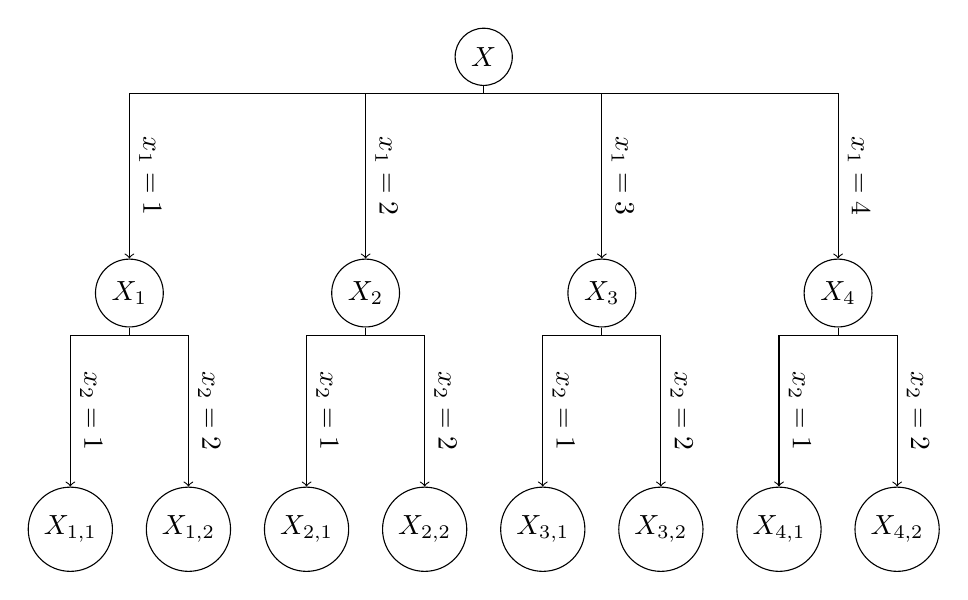
\begin{tikzpicture}[every child node/.style={circle,draw},level 1/.style={sibling distance=3cm},level 2/.style={sibling distance=1.5cm}, level distance = 3cm,edge from parent path={
(\tikzparentnode.south) |-   % Start from parent
++(0,-1mm) -|
    %($(\tikzparentnode.south)-(0,1mm)$) -|
%($(\tikzparentnode)!0.5!(\tikzchildnode)$) -| % make an ortho line to mid point
(\tikzchildnode.north)}]
        \node[circle,draw] (X) {$X$} 
	    child { node {$X_1$}
        	child { node {$X_{1,1}$} edge from parent [->] node (x2) [near end,above,sloped] {$x_2=1$} }
        	child { node {$X_{1,2}$} edge from parent [->] node (x2) [near end,above,sloped] {$x_2=2$} }
        	edge from parent [->] node [near end,above,sloped] (x1) {$x_1=1$}
            }
            child { node {$X_2$}
        	child { node {$X_{2,1}$} edge from parent [->] node [near end,above,sloped] {$x_2=1$} }
        	child { node {$X_{2,2}$} edge from parent [->] node [near end,above,sloped] {$x_2=2$} }
        	edge from parent [->] node [near end,above,sloped] {$x_1=2$}
            }
            child { node {$X_3$}
        	child { node {$X_{3,1}$} edge from parent [->] node [near end,above,sloped] {$x_2=1$} }
        	child { node {$X_{3,2}$} edge from parent [->] node [near end,above,sloped] {$x_2=2$} }
        	edge from parent [->] node [near end,above,sloped] {$x_1=3$}
            }
	    child { node {$X_4$}
        	child { node {$X_{4,1}$} edge from parent [->] node [near end,above,sloped] {$x_2=1$} }
        	child { node {$X_{4,2}$} edge from parent [->] node [near end,above,sloped] {$x_2=2$} }
        	edge from parent [->] node [near end,above,sloped] {$x_1=4$}
            }
            ;
	%\node[left = of x2] (x2_label) {$x_2=$};
	%\node at (x2_label |- x1) {$x_1=$};
	% \node[left = of x1 -| x2] {$x_1=$};
    \end{tikzpicture}
    \caption{Enumeration of all possible assignments for the integer variables of the example MILP problem of Eq. \eqref{eq:example-milp}, assuming lower and upper bounds are known. Leaf nodes contain the sets resulting from fixing the assignments, such that $X=X_1\cup \ldots\cup X_8$.}
    \label{fig:naive-tree-example-milp}
\end{figure}

As the leaf nodes of the enumeration tree are associated to feasible regions that contain a single possible value to all integer variables, the complete enumeration strategy leads to a decomposition of the problem into LP subproblems.
Therefore, it would be possible to compute an optimal solution (if it exists) for each subproblem in polynomial time.
However, this enumeration would only be possible if the problem is bounded in the integer variables.
On top of that, the number of leaf nodes grows exponentially with the size of the problem\footnotemark.
\footnotemark{In this context, the size of the problem is measured as the number of binary variables that the equivalent reformulation as a binary MILP would contain. The number of leaf nodes grows exponentially (with base 2) with respect to the number of such binary variables.}
Therefore, it is easy to see that the complete enumeration strategy is not a viable option even for problems of moderate size.

The branch-and-bound implements a guided exploration of the complete tree of integer assignments to avoid getting to the leaf nodes.
This guided exploration ignores (or \emph{prunes}) entire branches of the tree based on upper and lower bounds of the subproblems.
Such bounds can be computed, for example, through the LP relaxation of the subproblem or from any feasible solution.
To see this, take a problem $P$ as in \eqref{eq:general-milp} and let $X_1,\ldots,X_K$ be a decomposition of the feasible region $X$.
Let $\underline{z}^{k}$ and $\overline{z}^{k}$ be lower and upper bounds to $z^{k}$, the optimum cost of subproblem $P^{(k)}$, for each $k$.
Then, $\underline{z}=\min_k \underline{z}^{k}$ and $\overline{z}=\min_k \overline{z}^{k}$ are lower and upper bounds of $z$, the optimum cost of $P$.
Finally, if $\underline{z}^{k} \ge \overline{z}$ for a given $k$, then the optimal solution of $P^{(k)}$ will not be an optimal solution of $P$, because it is guaranteed that another subproblem has a better feasible solution.
In other words, even though the optimal solution of $P^{(k)}$ was not computed, it is possible to disregard $X_k$ in the decomposition, i.e., the respective branch can be entirely pruned. 

Again on the example MILP problem of \eqref{eq:example-milp}, suppose the LP relaxation of the root problem was solved, which resulted in a lower bound $\underline{z}=2.5$.
Then, a decomposition based on variable $x_2$ was made, such that $X=X_1\cup X_2$, with $X_k = \left\{ \bm{x} : A\bm{x}\le \bm{b}, x_2 = k \right\}$.
The LP relaxation of each $P^{(k)}$ resulted in lower and upper bounds as annotated in Fig.~\ref{fig:pruning-example-milp}.
Because the lower bound of $P^{(1)}$ is greater than the original problem's best known upper bound (as $\overline{z}=\min_k \overline{z}^{k}$), the optimal solution is definitely not in $X_1$, so this branch of the tree can be pruned (represented by the red accent in the figure).
Beyond that, the optimal solution of the LP relaxation $P^{(1)}$ is already an integer solution, so no further decomposition is necessary. 

\begin{figure}[h]
    \centering
    \begin{tikzpicture}[every child node/.style={circle,draw},level 1/.style={sibling distance=3cm},level 2/.style={sibling distance=1.5cm}, level distance = 3cm,edge from parent path={
(\tikzparentnode.south) |-   % Start from parent
++(0,-5mm) -|
    %($(\tikzparentnode.south)-(0,1mm)$) -|
%($(\tikzparentnode)!0.5!(\tikzchildnode)$) -| % make an ortho line to mid point
(\tikzchildnode.north)}]
        \node[circle,draw] (X) {$X$} 
	    child { node[fill=red!50] (X1) {$X_1$}
        	edge from parent [->] node [near end,above,sloped] (x1) {$x_2=1$}
            }
            child { node (X2) {$X_2$}
        	edge from parent [->] node [near end,above,sloped] {$x_2=2$}
            }
            ;
	\node[below left = 0cm of X] {$-2.5$} ;
	\node[above left = 0cm of X] {$-2$} ;
	\node[below left = 0cm of X1] {$-1$} ;
	\node[above left = 0cm of X1] {$-1$} ;
	\node[below left = 0cm of X2] {$-2.5$} ;
	\node[above left = 0cm of X2] {$-2$} ;
	%\node[left = of x2] (x2_label) {$x_2=$};
	%\node at (x2_label |- x1) {$x_1=$};
	% \node[left = of x1 -| x2] {$x_1=$};
    \end{tikzpicture}
    \caption{Example of tree exploration with MILP problem of Eq. \eqref{eq:example-milp}. Associated upper (resp. lower) bounds are illustrated at the top (resp. bottom) left of each node. Node of set $X_1$ is painted red to indicate it is pruned based on the bounds from $P^{(2)}$, which update the best known bounds of the root problem.}
    \label{fig:pruning-example-milp}
\end{figure}

Pruning the 

From what has been exposed, three rules can be listed that lead to prunning of the branch associated to a set $X_k$:
\begin{itemize}
    \item[Optimality] Subproblem $P^{(k)}$ was solved to optimality (e.g., through its LP relaxation having an optimal solution that respects the integrality constraints);
    \item[Bound] The associated lower bound $\underline{z}^{k}$ is higher than $\overline{z}^{k}$ ;
    \item[Infeasibility] $X_k = \varnothing$.
\end{itemize}


% As Fig.~\ref{fig:milp-example} illustrates, the optimal solutions to this problem are $\bm{x}^{*} \in \left\{ (2,2),(3,2) \right\} $, whereas the optimal solution of its LP relaxation is $(2.5, 2.5)$. 






The main idea behind the branch-and-bound algorithm is to ignore the integrality constraints of the MILP problem, solve the resulting LP, and hope that the solution has the necessary integer components~\cite{vanderbeiLinearProgrammingFoundations1998}.
If the LP relaxation\footnote{The linear programming problem obtained by ignoring the integrality constraints of an MILP is called its \emph{LP relaxation}.} of an MILP problem has an optimal solution that respects the integrality constraints, than that solution is also optimal for the original problem.
% integer solutions are naturally occuring to the LP problem on the convex hull of integer solutions for an MILP
% this is easy to see, as optimal solutions (if they exist) to LPs are always at the vertices of its feasible region (which is a polytope) and the vertices of the convex hull of an MILP all respect the original integrality constraints
However, that is not always the case.
As an example, take the MILP problem

\begin{figure}[h]
    \centering
    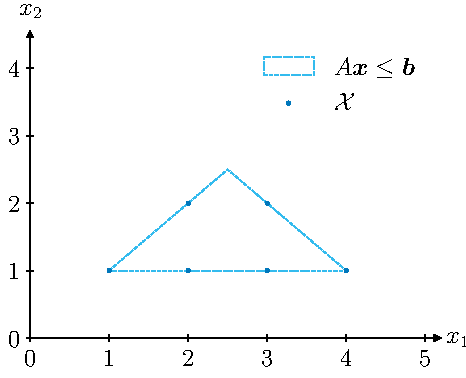
\includegraphics{pictures/milp_example_feasible_region.pdf}
    \caption{Feasible region of example MILP problem \eqref{eq:example-milp}. Dashed lines represent the feasible region of the LP relaxation.}
    \label{fig:milp-example}
\end{figure}

A naïve approach is to round the solution of the LP relaxation to the nearest integer value on the variables that violate the integrality constraints.
This strategy, however, might not even result in feasible solutions to the LP relaxation.
Note that an optimal solution to an LP is at a vertex of its feasible region, and, thus, a naïve deviation can result in an infeasible solution.

One way to guarantee that the solution to the LP relaxation will be the optimal solution to the MILP problem is to constrain the feasible region of the LP to be the \emph{convex hull} of $X$.
In other words, given an MILP problem such as in \eqref{eq:general-milp}, the solution to the LP problem
\begin{align*}
    \min_{\bm{x}} \quad & \bm{c}^{T}\bm{x} \\
    \textrm{s.t.} \quad & \bm{x}\in \conv(X) \times  \R^{n+p}
\end{align*}
is guaranteed to be the optimal solution to the original problem.



\subsection{Heuristics}

\subsection{Matheuristics}

